




\begin{figure}[h]
\begin{center}
	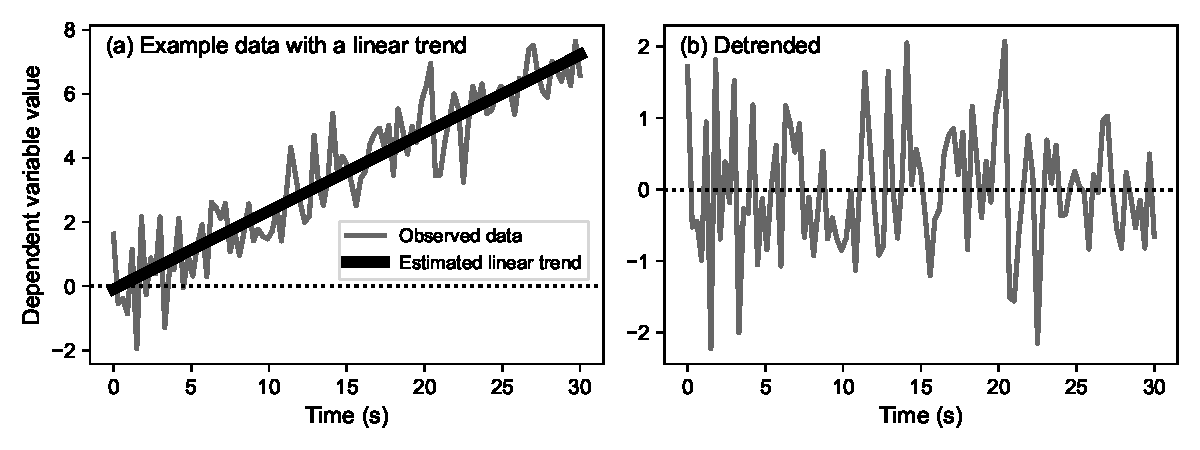
\includegraphics[width=0.99\textwidth]{./figs/fig_common.pdf}\vspace{0mm}
	\caption[Dummy caption.]{Common detrending example.}
	\label{fig:common}
\end{center}
\end{figure}



\begin{figure}[h]
\begin{center}
	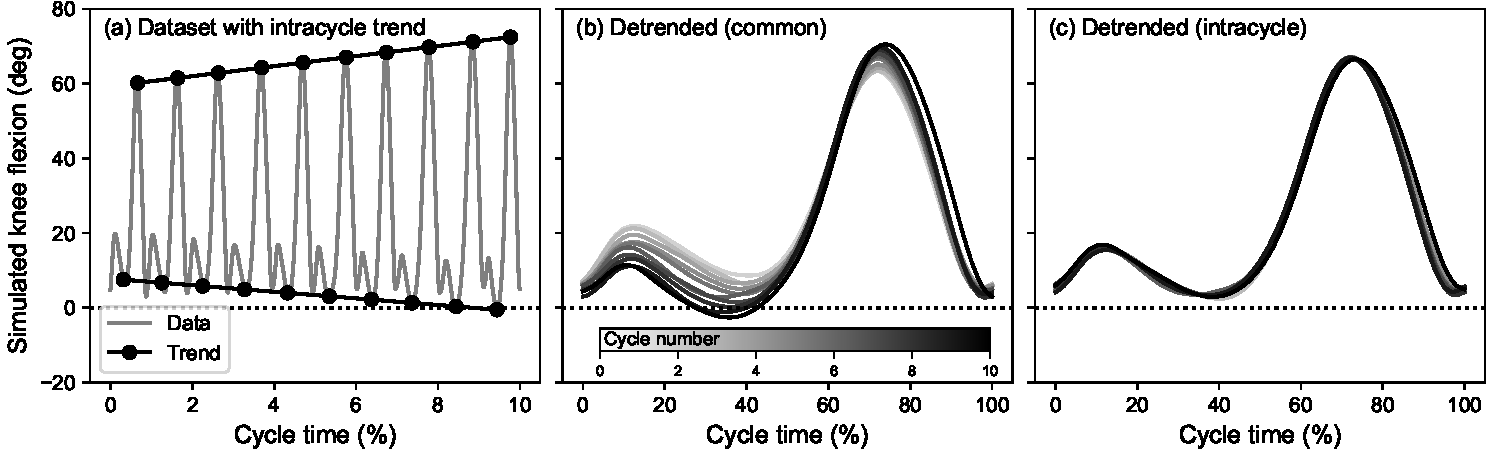
\includegraphics[width=0.99\textwidth]{./figs/fig_intracycle.pdf}\vspace{0mm}
	\caption[Dummy caption.]{Example intracycle trend with detrending results.}
	\label{fig:intracycle}
\end{center}
\end{figure}



\begin{figure}[h]
\begin{center}
	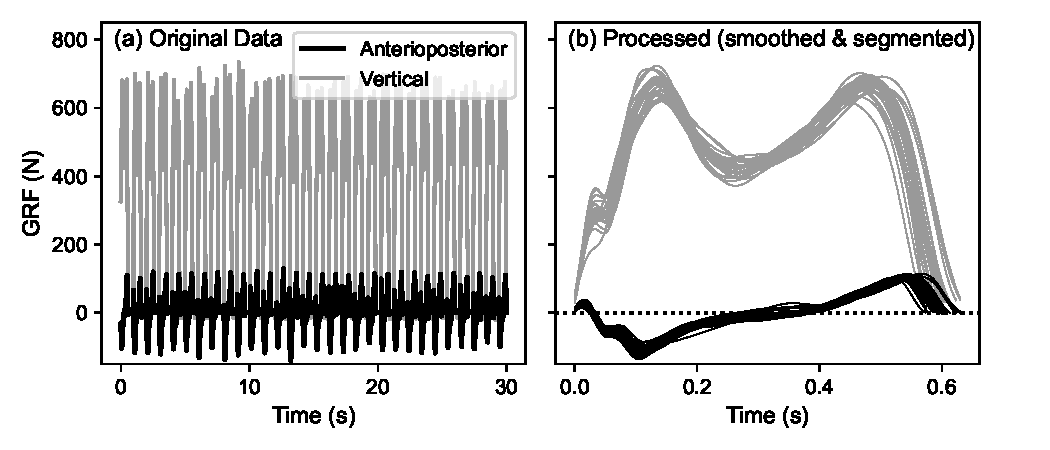
\includegraphics[width=0.99\textwidth]{./figs/fig_grf_dataset.pdf}\vspace{0mm}
	\caption[Dummy caption.]{Experimental dataset from Fukuchi et al. (2018).}
	\label{fig:grf_dataset}
\end{center}
\end{figure}




\begin{figure}[h]
\begin{center}
	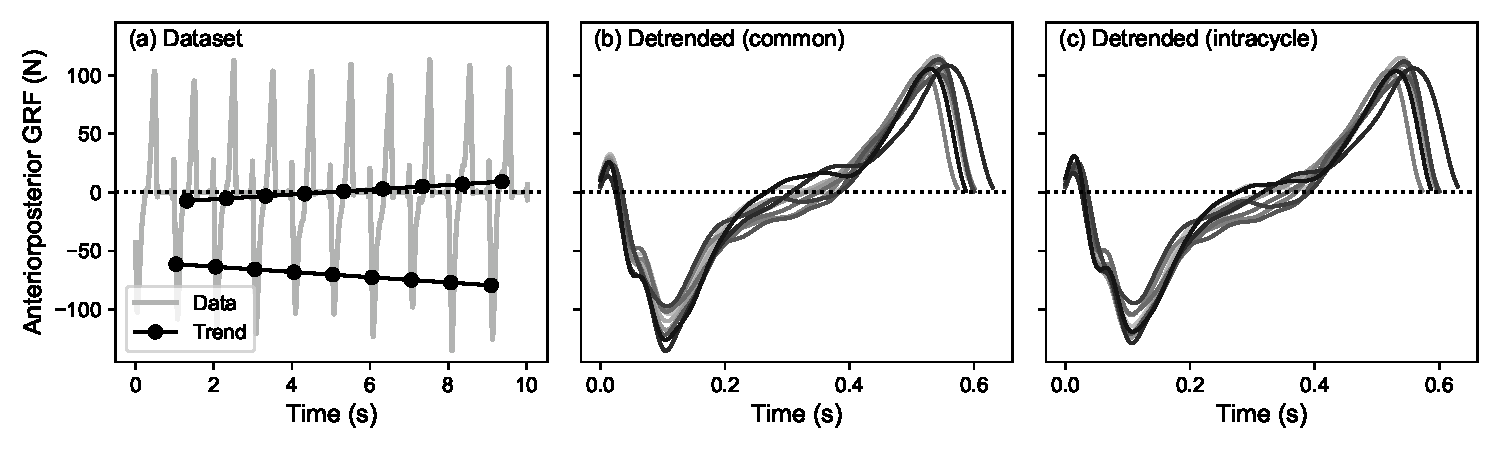
\includegraphics[width=0.99\textwidth]{./figs/fig_results_detrend.pdf}\vspace{0mm}
	\caption[Dummy caption.]{Detrending results for the experimental GRF dataset.}
	\label{fig:results_detrend}
\end{center}
\end{figure}



\begin{figure}[h]
\begin{center}
	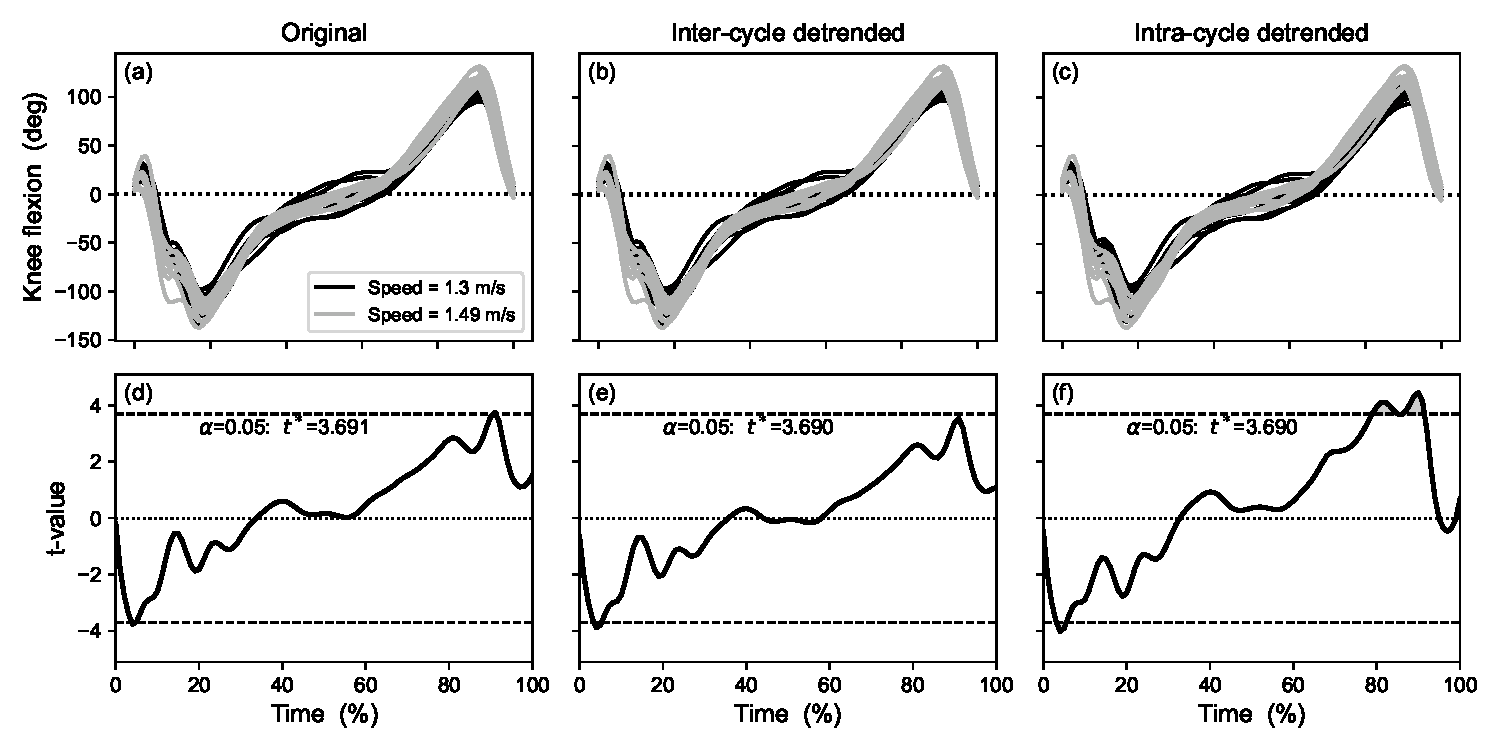
\includegraphics[width=0.99\textwidth]{./figs/fig_spm_01.pdf}\vspace{0mm}
	\caption[Dummy caption.]{Two-sample t-test results for speeds = 1.3 and 1.49 m/s.}
	\label{fig:spm01}
\end{center}
\end{figure}


\begin{figure}[h]
\begin{center}
	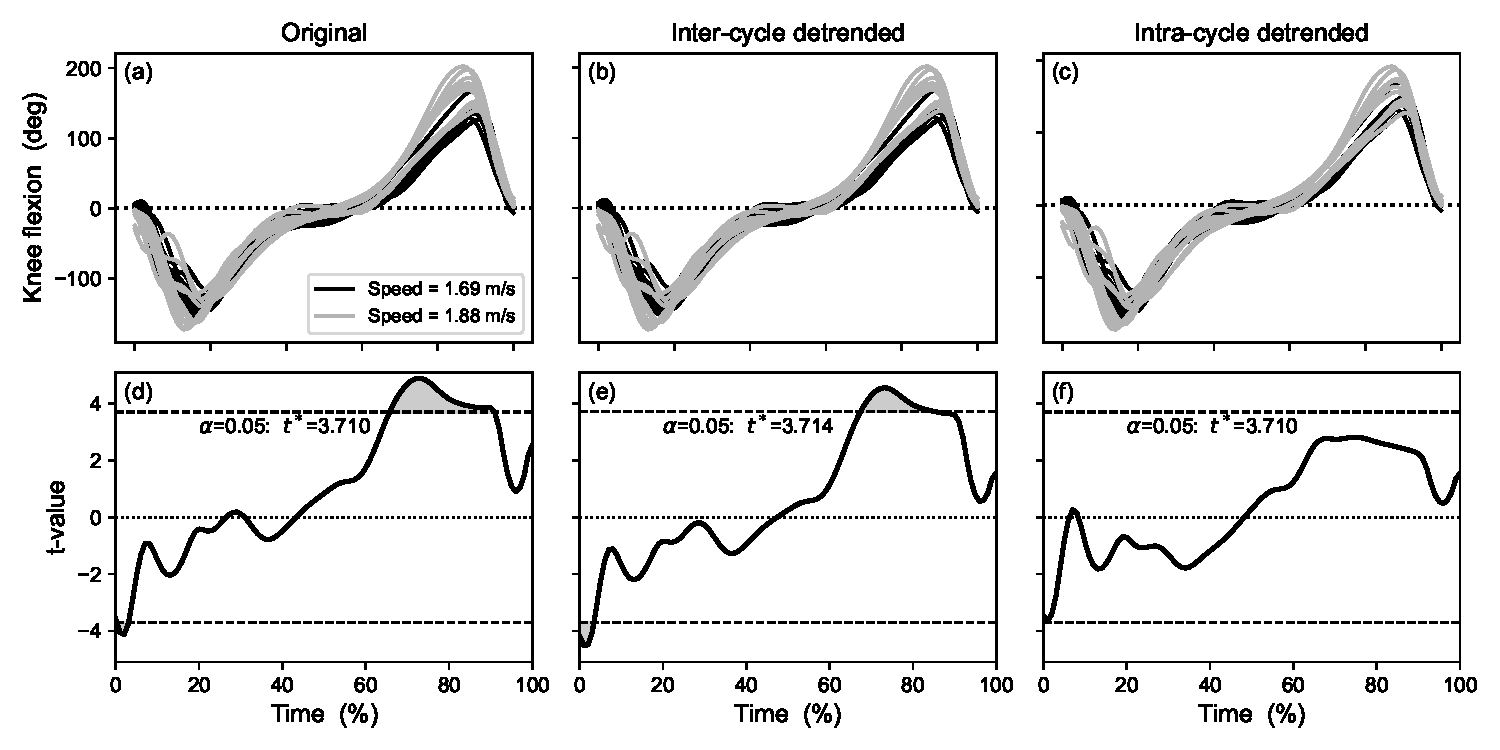
\includegraphics[width=0.99\textwidth]{./figs/fig_spm_23.pdf}\vspace{0mm}
	\caption[Dummy caption.]{Two-sample t-test results for speeds = 1.69 and 1.88 m/s.}
	\label{fig:spm23}
\end{center}
\end{figure}
